%%%%%%%%%%%%%%%%%%%%%%%%%%%%%%%%%%%%%%%%%
% Lachaise Assignment
% LaTeX Template
% Version 1.0 (26/6/2018)
%
% This template originates from:
% http://www.LaTeXTemplates.com
%
% Authors:
% Marion Lachaise & François Févotte
% Vel (vel@LaTeXTemplates.com)
%
% License:
% CC BY-NC-SA 3.0 (http://creativecommons.org/licenses/by-nc-sa/3.0/)
% 
%%%%%%%%%%%%%%%%%%%%%%%%%%%%%%%%%%%%%%%%%

%----------------------------------------------------------------------------------------
%	PACKAGES AND OTHER DOCUMENT CONFIGURATIONS
%----------------------------------------------------------------------------------------

\documentclass{article}

%%%%%%%%%%%%%%%%%%%%%%%%%%%%%%%%%%%%%%%%%
% Lachaise Assignment
% Structure Specification File
% Version 1.0 (26/6/2018)
%
% This template originates from:
% http://www.LaTeXTemplates.com
%
% Authors:
% Marion Lachaise & François Févotte
% Vel (vel@LaTeXTemplates.com)
%
% License:
% CC BY-NC-SA 3.0 (http://creativecommons.org/licenses/by-nc-sa/3.0/)
% 
%%%%%%%%%%%%%%%%%%%%%%%%%%%%%%%%%%%%%%%%%

%----------------------------------------------------------------------------------------
%	PACKAGES AND OTHER DOCUMENT CONFIGURATIONS
%----------------------------------------------------------------------------------------

\usepackage{amsmath,amsfonts,stmaryrd,amssymb} % Math packages

\usepackage{enumerate} % Custom item numbers for enumerations

\usepackage[ruled]{algorithm2e} % Algorithms

\usepackage[framemethod=tikz]{mdframed} % Allows defining custom boxed/framed environments

\usepackage{listings} % File listings, with syntax highlighting
\lstset{
	basicstyle=\ttfamily, % Typeset listings in monospace font
}

%----------------------------------------------------------------------------------------
%	DOCUMENT MARGINS
%----------------------------------------------------------------------------------------

\usepackage{geometry} % Required for adjusting page dimensions and margins

\geometry{
	paper=a4paper, % Paper size, change to letterpaper for US letter size
	top=2.5cm, % Top margin
	bottom=3cm, % Bottom margin
	left=2.5cm, % Left margin
	right=2.5cm, % Right margin
	headheight=14pt, % Header height
	footskip=1.5cm, % Space from the bottom margin to the baseline of the footer
	headsep=1.2cm, % Space from the top margin to the baseline of the header
	%showframe, % Uncomment to show how the type block is set on the page
}

%----------------------------------------------------------------------------------------
%	FONTS
%----------------------------------------------------------------------------------------

\usepackage[utf8]{inputenc} % Required for inputting international characters
\usepackage[T1]{fontenc} % Output font encoding for international characters
\usepackage{etoolbox} % Required for if statements
\usepackage[brazil]{babel}
\usepackage{mathtools}
\usepackage{float}


\usepackage{XCharter} % Use the XCharter fonts

%----------------------------------------------------------------------------------------
%	COMMAND LINE ENVIRONMENT
%----------------------------------------------------------------------------------------

% Usage:
% \begin{commandline}
%	\begin{verbatim}
%		$ ls
%		
%		Applications	Desktop	...
%	\end{verbatim}
% \end{commandline}

\mdfdefinestyle{commandline}{
	leftmargin=10pt,
	rightmargin=10pt,
	innerleftmargin=15pt,
	middlelinecolor=black!50!white,
	middlelinewidth=2pt,
	frametitlerule=false,
	backgroundcolor=black!5!white,
	frametitle={Command Line},
	frametitlefont={\normalfont\sffamily\color{white}\hspace{-1em}},
	frametitlebackgroundcolor=black!50!white,
	nobreak,
}

% Define a custom environment for command-line snapshots
\newenvironment{commandline}{
	\medskip
	\begin{mdframed}[style=commandline]
}{
	\end{mdframed}
	\medskip
}

%----------------------------------------------------------------------------------------
%	FILE CONTENTS ENVIRONMENT
%----------------------------------------------------------------------------------------

% Usage:
% \begin{file}[optional filename, defaults to "File"]
%	File contents, for example, with a listings environment
% \end{file}

\mdfdefinestyle{file}{
	innertopmargin=1.6\baselineskip,
	innerbottommargin=0.8\baselineskip,
	topline=false, bottomline=false,
	leftline=false, rightline=false,
	leftmargin=2cm,
	rightmargin=2cm,
	singleextra={%
		\draw[fill=black!10!white](P)++(0,-1.2em)rectangle(P-|O);
		\node[anchor=north west]
		at(P-|O){\ttfamily\mdfilename};
		%
		\def\l{3em}
		\draw(O-|P)++(-\l,0)--++(\l,\l)--(P)--(P-|O)--(O)--cycle;
		\draw(O-|P)++(-\l,0)--++(0,\l)--++(\l,0);
	},
	nobreak,
}

% Define a custom environment for file contents
\newenvironment{file}[1][File]{ % Set the default filename to "File"
	\medskip
	\newcommand{\mdfilename}{#1}
	\begin{mdframed}[style=file]
}{
	\end{mdframed}
	\medskip
}

%----------------------------------------------------------------------------------------
%	NUMBERED QUESTIONS ENVIRONMENT
%----------------------------------------------------------------------------------------

% Usage:
% \begin{question}[optional title]
%	Question contents
% \end{question}

\mdfdefinestyle{question}{
	innertopmargin=1.2\baselineskip,
	innerbottommargin=0.8\baselineskip,
	roundcorner=5pt,
	nobreak,
	singleextra={%
		\draw(P-|O)node[xshift=1em,anchor=west,fill=white,draw,rounded corners=5pt]{%
		Question \theQuestion\questionTitle};
	},
}

\newcounter{Question} % Stores the current question number that gets iterated with each new question

% Define a custom environment for numbered questions
\newenvironment{question}[1][\unskip]{
	\bigskip
	\stepcounter{Question}
	\newcommand{\questionTitle}{~#1}
	\begin{mdframed}[style=question]
}{
	\end{mdframed}
	\medskip
}

%----------------------------------------------------------------------------------------
%	WARNING TEXT ENVIRONMENT
%----------------------------------------------------------------------------------------

% Usage:
% \begin{warn}[optional title, defaults to "Warning:"]
%	Contents
% \end{warn}

\mdfdefinestyle{warning}{
	topline=false, bottomline=false,
	leftline=false, rightline=false,
	nobreak,
	singleextra={%
		\draw(P-|O)++(-0.5em,0)node(tmp1){};
		\draw(P-|O)++(0.5em,0)node(tmp2){};
		\fill[black,rotate around={45:(P-|O)}](tmp1)rectangle(tmp2);
		\node at(P-|O){\color{white}\scriptsize\bf !};
		\draw[very thick](P-|O)++(0,-1em)--(O);%--(O-|P);
	}
}

% Define a custom environment for warning text
\newenvironment{warn}[1][Warning:]{ % Set the default warning to "Warning:"
	\medskip
	\begin{mdframed}[style=warning]
		\noindent{\textbf{#1}}
}{
	\end{mdframed}
}

%----------------------------------------------------------------------------------------
%	INFORMATION ENVIRONMENT
%----------------------------------------------------------------------------------------

% Usage:
% \begin{info}[optional title, defaults to "Info:"]
% 	contents
% 	\end{info}

\mdfdefinestyle{info}{%
	topline=false, bottomline=false,
	leftline=false, rightline=false,
	nobreak,
	singleextra={%
		\fill[black](P-|O)circle[radius=0.4em];
		\node at(P-|O){\color{white}\scriptsize\bf i};
		\draw[very thick](P-|O)++(0,-0.8em)--(O);%--(O-|P);
	}
}

% Define a custom environment for information
\newenvironment{info}[1][Info:]{ % Set the default title to "Info:"
	\medskip
	\begin{mdframed}[style=info]
		\noindent{\textbf{#1}}
}{
	\end{mdframed}
}
 % Include the file specifying the document structure and custom commands

%----------------------------------------------------------------------------------------
%	ASSIGNMENT INFORMATION
%----------------------------------------------------------------------------------------

\title{MAE001: Modelagem Matemática em Finanças I} % Title of the assignment

\author{Ramon Duarte de Melo\\ \texttt{ramonduarte@poli.ufrj.br} % Author name and email address
\\ Alex Teixeira\\ \texttt{ramonduarte@poli.ufrj.br}} % Author name and email address

\date{Universidade Federal do Rio de Janeiro (UFRJ) --- \today} % University, school and/or department name(s) and a date

%----------------------------------------------------------------------------------------

\begin{document}

\maketitle % Print the title

%----------------------------------------------------------------------------------------
%	INTRODUCTION
%----------------------------------------------------------------------------------------

\section*{Introdução} % Unnumbered section

O objetivo do Projeto III é implementar, avaliar e comparar o modelo de Black-Scholes com os dados fornecidos pelo mundo real, realizando comparações de cunho matemático-estatístico e produzindo gráficos com tais observações acerca da volatilidade implícita, do preço de corte (\emph{strike price} e dos recortes temporais). 

Para tal, foi utilizada a linguagem \emph{Python 3.6.7}, com os módulos \emph{numpy} (métodos numéricos), \emph{pandas} (manipulação de dados), \emph{scipy} (fórmulas científicas) e \emph{matplotlib.pyplot} (visualização de dados).

Os dados utilizados para a confecção das comparações foi raspado da web utilizando as ferramentas \emph{bs4} (web parsing), \emph{lxml} (HTML parsing) e \emph{re} (expressões regulares). O programa requer a instalação destes módulos, mas possui uma ferramenta de instalação automatizada das dependências (\emph{pipenv}). 

As fontes dos dados são a B3 (Brasil Bolsa Balcão, operadora da Bolsa de Valores de São Paulo) e o jornal Valor Econômico. Todos os dados são referentes ao mercado logo após o fechamento (17:00) do dia 6º de junho de 2019. O ativo utilizado, \textbf{PETR4 ON}, fechou o pregão a $R\$ $ $29,85$.


O código utilizado neste trabalho, bem como o deste relatório e as imagens geradas, foi aberto e disponibilizado publicamente no repositório https://github.com/ramonduarte/mmftrab3.


%----------------------------------------------------------------------------------------
%	PROBLEM 1
%----------------------------------------------------------------------------------------

\section*{Atividade \emph{a}} % Numbered section

Nesta atividade, foi implementado o modelo de Black-Scholes da seguinte forma:

\begin{enumerate}
	\item Conforme definição, o modelo de Black-Scholes define preços de opções como uma função do preço do ativo subjacente $S$, do preço de execução $K$ (também chamado de \emph{strike price}), da taxa de renda fixa $r$ (aqui foi usada a Taxa Selic), do tempo até o prazo de execução $t$ e da volatilidade $\sigma$.
	
	\[V = BS(S,K,r,T,\sigma)\]

	\item Como todos os valores acima são conhecidos exceto a volatilidade, é possível descrever o preço da opção como uma função somente dela.
		
	\[V = BS(\sigma)\]

	\item Para tanto, é necessário descobrir o valor da opção $V$. Como o modelo de Black-Scholes apoia-se na premissa da \emph{informação perfeita}, podemos considerar que toda opção negociada na bolsa de valores está decentemente precificada.
	\item No entanto, não é possível manipular a equação de Black-Scholes para isolar o valor da volatilidade, de forma que a única maneira de calculá-la é utilizar a técnica de bisseção. 
\end{enumerate}

Com os valores obtidos, foram gerados gráficos $K \times T$ para opções de compra e venda do ativo \textbf{PETR4\ ON} para exercício em três datas: 17/06/2019, 19/08/2019 e 20/01/2020, respectivamente.
As opções não foram separadas entre derivativos europeus e americanos.
No entanto, somente foram incluídos derivativos europeus e americanos.
Contratos exóticos e/ou dependentes de caminho não foram incluídos.



\begin{figure}[]
	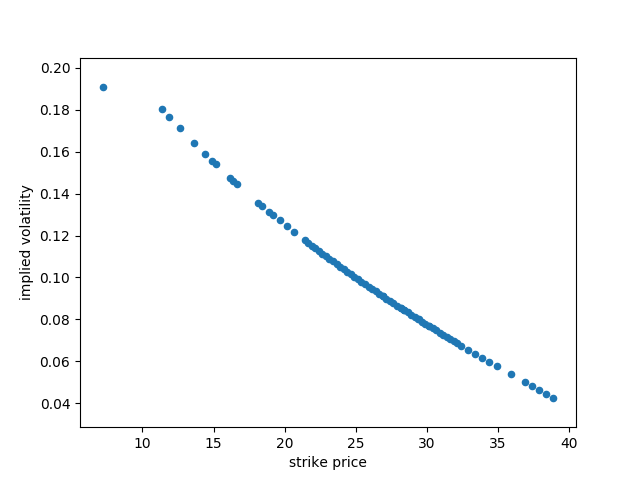
\includegraphics[width=0.9\linewidth]{Figure_0.png}
	\centering
	
	\caption{Gráfico $K \times \sigma$ para opções do ativo \textbf{PETR4 ON} com data de exercício 17/06/2019.}
	\label{}
\end{figure}

\begin{figure}[]
	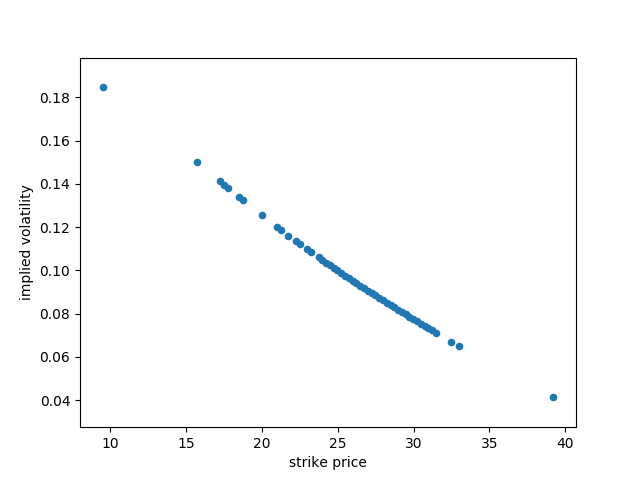
\includegraphics[width=0.9\linewidth]{Figure_1.png}
	\centering
	
	\caption{Gráfico $K \times \sigma$ para opções do ativo \textbf{PETR4 ON} com data de exercício 19/08/2019.}
	\label{}
\end{figure}

\begin{figure}[]
	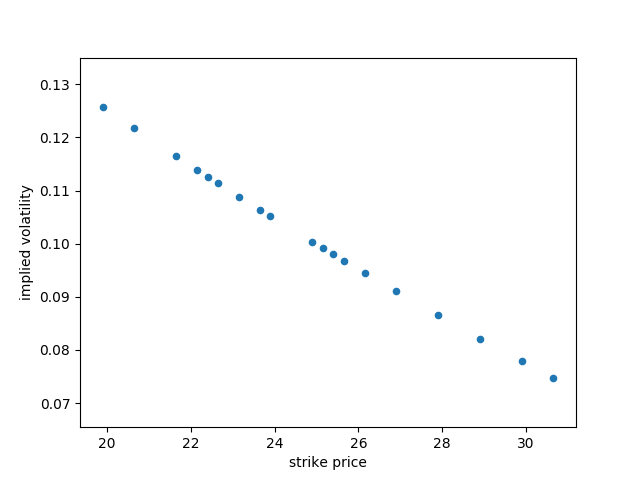
\includegraphics[width=0.9\linewidth]{Figure_2.png}
	\centering
	
	\caption{Gráfico $K \times \sigma$ para opções do ativo \textbf{PETR4 ON} com data de exercício 20/01/2020.}
	\label{}
\end{figure}

%----------------------------------------------------------------------------------------
%	PROBLEM 2
%----------------------------------------------------------------------------------------


\section*{Atividade \emph{b}}

Para esta atividade, o processo utilizado foi o mesmo do da anterior.
As únicas mudanças foram:

\begin{itemize}
	\item Uma subbiblioteca do \emph{matplotlib}, externa ao \emph{pyplot}, teve de ser utilizada para gerar o gráfico em 3D, porque o \emph{pyplot} não gera gráficos 3D interativos, necessários para a escolha da melhor perspectiva.
	\item Todas as opções encontradas para o ativo \textbf{PETR4 ON} foram utilizadas, desde que estivessem precificadas após o fechamento do pregão da Bolsa de Valores de São Paulo em 06/06/2019.
\end{itemize}

\begin{figure}[H]
	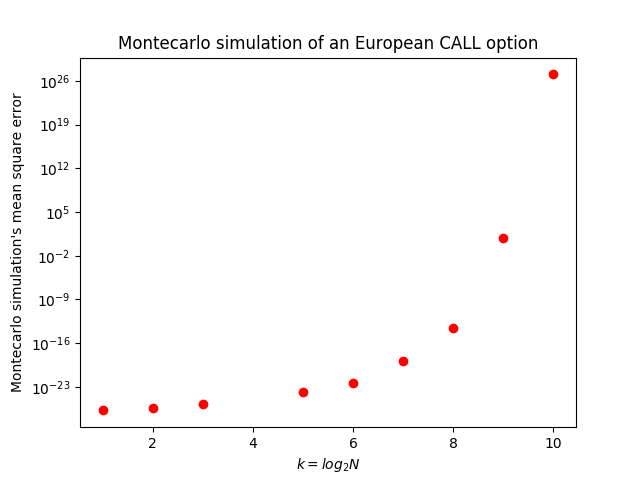
\includegraphics[width=\linewidth]{Figure_3.png}
	\centering
	
	\caption{\textbf{Superfície de volatilidade}: séries $K \times \sigma$ separadas por data de exercício.}
	\label{}
\end{figure}

%----------------------------------------------------------------------------------------
%	PROBLEM 2
%----------------------------------------------------------------------------------------

\section*{Atividade c}

Com exceção da \emph{Figura 3}, foi possível enxergar o \emph{smile} em todos os gráficos plotados.
Como o ativo \textbf{PETR4 ON} é bastante negociado na bolsa de valores, suas distribuições tendem a se aproximarem do previsto pelo modelo teórico.
É justamente por isso que, na \emph{Figura 3}, a observação do \emph{smile} é mais difícil, pois as opções com exercício nesta data - mais distante - são menos negociadas e, portanto, não formam pontos suficientes para a construção da curva com visibilidade.

Na \emph{Figura 4}, inclusive, é possível notar a formação de várias curvas deste tipo ao longo das datas de exercício, bem como seu rareamento conforme o aumento do prazo.


\end{document}
